\subsection{Overview}

Xamarin is a mobile app development framework targeting iOS and Android primarily. It was founded in 2011 (\cite{de_icaza_announcing_2011}) and sold to Microsoft in 2016, after managing to acquire more than 15.000 customers in 120 countries in its previous five years of existence, including 20\% of the Fortune 500 companies and 1.3 million unique developers (\cite{guthrie_microsoft_2016}).

\begin{figure}[H]
\centering
\caption{The Xamarin Products}
\label{fig:chasm}
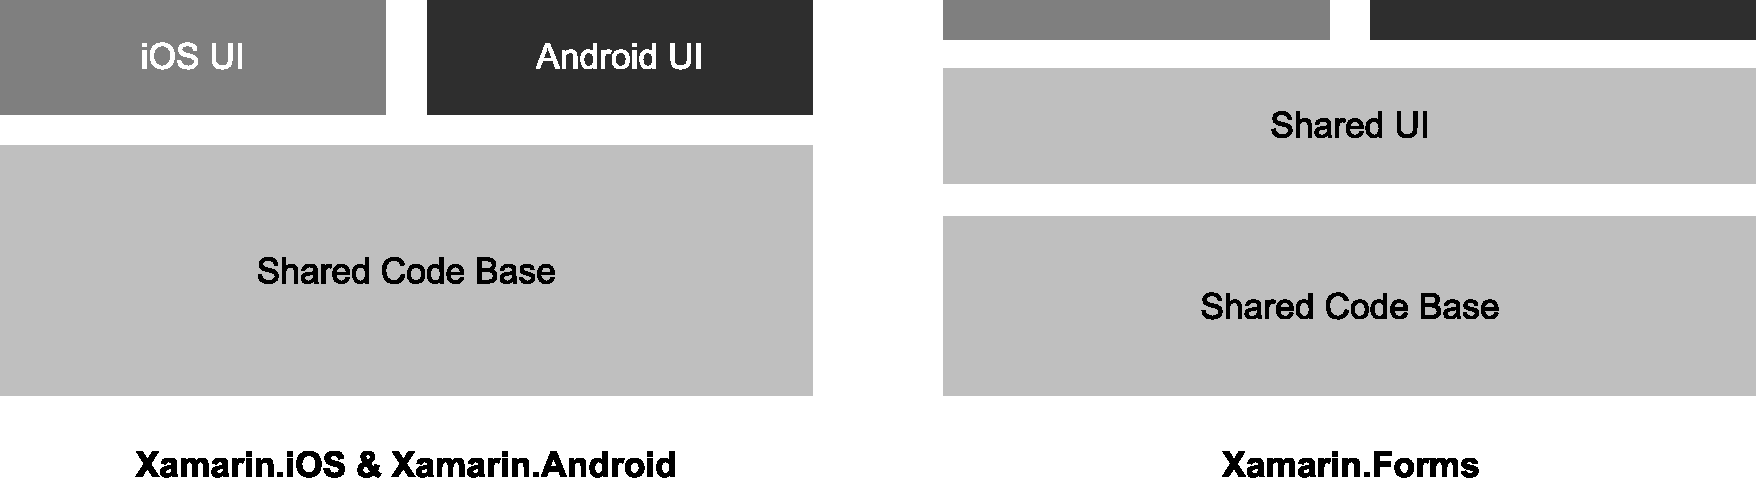
\includegraphics[width=\textwidth]{xamarin}
\source{Own illustration}
\end{figure}

Its key feature is to enable developers to share code written in any .NET language across multiple platforms (\cite[6]{petzold_creating_2016}). This is not only true for code running on Apple's mobile operating systems and Android, but also on other platforms like Windows, macOS, or Linux. This enables code sharing between mobile clients and the backend, which can be especially useful for apps that, for example, must work offline. 

Its direct competition can be categorized as two-fold. Its two core products, Xamarin.iOS and Xamarin.Android compete with native implementation approaches like writing apps in Swift or Java, its third product Xamarin.Forms is in a fierce competition with React Native and Flutter (\cite[9]{kuitunen_cross-platform_2019}; \cite[9]{fayzullaev_native-like_2018}).

Xamarin.Forms provides a comprehensive UI toolkit on top of both platforms. It enables developers to share not only code for business logic and infrastructure tasks, but also the user interface. Which is especially attractive for line of business applications and also for any developer who wants to prototype and test their ideas fast while still delivering a native user experience.
